% presentation_pitch_3min.tex
% =====================================================================
% Pitch de 3 minutes, pour un auditoire qui ne connait PAS le sujet.
%
% Parti pris : expliquer les concepts et l'avancement, pas enumerer des
% resultats. Chaque slide pose une notion avant de s'en servir, et chaque
% chiffre arrive apres le dispositif qui le produit. Les chiffres detailles
% de C.1, C.2 et C.3 sont volontairement absents : chacun exige sa
% definition prealable, et trois minutes ne les financent pas.
%
% Les resultats s'arretent a la fin de la question C. La question D est
% annoncee comme le travail suivant, et aucun chiffre des
% `redaction_QD*.tex` n'apparait ici.
%
% Compilation :  latexmk -lualatex presentation_pitch_3min.tex
% (metropolis charge les fontes Fira, ce que pdflatex ne fait pas.)
%
% Tracabilite des chiffres :
%   ../04_experimentations/resultats_R2/scripts/chiffres_slides.py
%       (les 3 alarmes de R2, et les six chiffres de C.1)
%   ../04_experimentations/resultats_R2/scripts/verif_chiffres_tex.py
%       ../../05_presentation/presentation_pitch_3min.tex
% Les figures sortent de resultats_R2/scripts/figures_slides.py.

\documentclass[aspectratio=169,11pt]{beamer}

\usetheme{metropolis}
\usepackage[english]{babel}
\usepackage{amsmath,amssymb}
\usepackage{graphicx}
\setbeamertemplate{navigation symbols}{}
% Sortie « notes seules », pour repeter :
%   lualatex "\def\NOTESSEULES{}% presentation_pitch_3min.tex
% =====================================================================
% Pitch de 3 minutes, pour un auditoire qui ne connait PAS le sujet.
%
% Parti pris : expliquer les concepts et l'avancement, pas enumerer des
% resultats. Chaque slide pose une notion avant de s'en servir, et chaque
% chiffre arrive apres le dispositif qui le produit. Les chiffres detailles
% de C.1, C.2 et C.3 sont volontairement absents : chacun exige sa
% definition prealable, et trois minutes ne les financent pas.
%
% Les resultats s'arretent a la fin de la question C. La question D est
% annoncee comme le travail suivant, et aucun chiffre des
% `redaction_QD*.tex` n'apparait ici.
%
% Compilation :  latexmk -lualatex presentation_pitch_3min.tex
% (metropolis charge les fontes Fira, ce que pdflatex ne fait pas.)
%
% Tracabilite des chiffres :
%   ../04_experimentations/resultats_R2/scripts/chiffres_slides.py
%       (les 3 alarmes de R2, et les six chiffres de C.1)
%   ../04_experimentations/resultats_R2/scripts/verif_chiffres_tex.py
%       ../../05_presentation/presentation_pitch_3min.tex
% Les figures sortent de resultats_R2/scripts/figures_slides.py.

\documentclass[aspectratio=169,11pt]{beamer}

\usetheme{metropolis}
\usepackage[english]{babel}
\usepackage{amsmath,amssymb}
\usepackage{graphicx}
\setbeamertemplate{navigation symbols}{}
% Sortie « notes seules », pour repeter :
%   lualatex "\def\NOTESSEULES{}% presentation_pitch_3min.tex
% =====================================================================
% Pitch de 3 minutes, pour un auditoire qui ne connait PAS le sujet.
%
% Parti pris : expliquer les concepts et l'avancement, pas enumerer des
% resultats. Chaque slide pose une notion avant de s'en servir, et chaque
% chiffre arrive apres le dispositif qui le produit. Les chiffres detailles
% de C.1, C.2 et C.3 sont volontairement absents : chacun exige sa
% definition prealable, et trois minutes ne les financent pas.
%
% Les resultats s'arretent a la fin de la question C. La question D est
% annoncee comme le travail suivant, et aucun chiffre des
% `redaction_QD*.tex` n'apparait ici.
%
% Compilation :  latexmk -lualatex presentation_pitch_3min.tex
% (metropolis charge les fontes Fira, ce que pdflatex ne fait pas.)
%
% Tracabilite des chiffres :
%   ../04_experimentations/resultats_R2/scripts/chiffres_slides.py
%       (les 3 alarmes de R2, et les six chiffres de C.1)
%   ../04_experimentations/resultats_R2/scripts/verif_chiffres_tex.py
%       ../../05_presentation/presentation_pitch_3min.tex
% Les figures sortent de resultats_R2/scripts/figures_slides.py.

\documentclass[aspectratio=169,11pt]{beamer}

\usetheme{metropolis}
\usepackage[english]{babel}
\usepackage{amsmath,amssymb}
\usepackage{graphicx}
\setbeamertemplate{navigation symbols}{}
% Sortie « notes seules », pour repeter :
%   lualatex "\def\NOTESSEULES{}% presentation_pitch_3min.tex
% =====================================================================
% Pitch de 3 minutes, pour un auditoire qui ne connait PAS le sujet.
%
% Parti pris : expliquer les concepts et l'avancement, pas enumerer des
% resultats. Chaque slide pose une notion avant de s'en servir, et chaque
% chiffre arrive apres le dispositif qui le produit. Les chiffres detailles
% de C.1, C.2 et C.3 sont volontairement absents : chacun exige sa
% definition prealable, et trois minutes ne les financent pas.
%
% Les resultats s'arretent a la fin de la question C. La question D est
% annoncee comme le travail suivant, et aucun chiffre des
% `redaction_QD*.tex` n'apparait ici.
%
% Compilation :  latexmk -lualatex presentation_pitch_3min.tex
% (metropolis charge les fontes Fira, ce que pdflatex ne fait pas.)
%
% Tracabilite des chiffres :
%   ../04_experimentations/resultats_R2/scripts/chiffres_slides.py
%       (les 3 alarmes de R2, et les six chiffres de C.1)
%   ../04_experimentations/resultats_R2/scripts/verif_chiffres_tex.py
%       ../../05_presentation/presentation_pitch_3min.tex
% Les figures sortent de resultats_R2/scripts/figures_slides.py.

\documentclass[aspectratio=169,11pt]{beamer}

\usetheme{metropolis}
\usepackage[english]{babel}
\usepackage{amsmath,amssymb}
\usepackage{graphicx}
\setbeamertemplate{navigation symbols}{}
% Sortie « notes seules », pour repeter :
%   lualatex "\def\NOTESSEULES{}\input{presentation_pitch_3min}"
\ifdefined\NOTESSEULES\setbeameroption{show only notes}\fi
\graphicspath{{../04_experimentations/resultats_R2/resultats/figures/}}

% Fontes resserrees pour que les quatre auteurs tiennent sur une ligne.
% (L'« Overfull vbox » de la page de titre vient du theme metropolis
% lui-meme : il se reproduit a l'identique avec un titre d'un seul
% caractere, et rien n'est coupe au rendu. Ne pas chercher a le corriger.)
\setbeamerfont{author}{size=\small}
\setbeamerfont{institute}{size=\scriptsize}

\title{The Blind Spot Paradox}
\subtitle{When a self-repairing model destroys the evidence its own monitor needs}
\author{Alexandre Boyer \and Mélaine Gouillou \and Salomé Fonvielle \and Ulysse Petit-Tichanné}
\institute{Research Track, Topic 39, CentraleSupélec. Supervisor: Raphaël Minato}
\date{}

\begin{document}

\maketitle
\note{The Blind Spot Paradox: when a self-repairing model destroys the
  evidence its own monitor needs.}

% ---------------------------------------------------------------- 32 s
\begin{frame}{Concept drift: the rule changes, the data does not}
  \begin{center}
    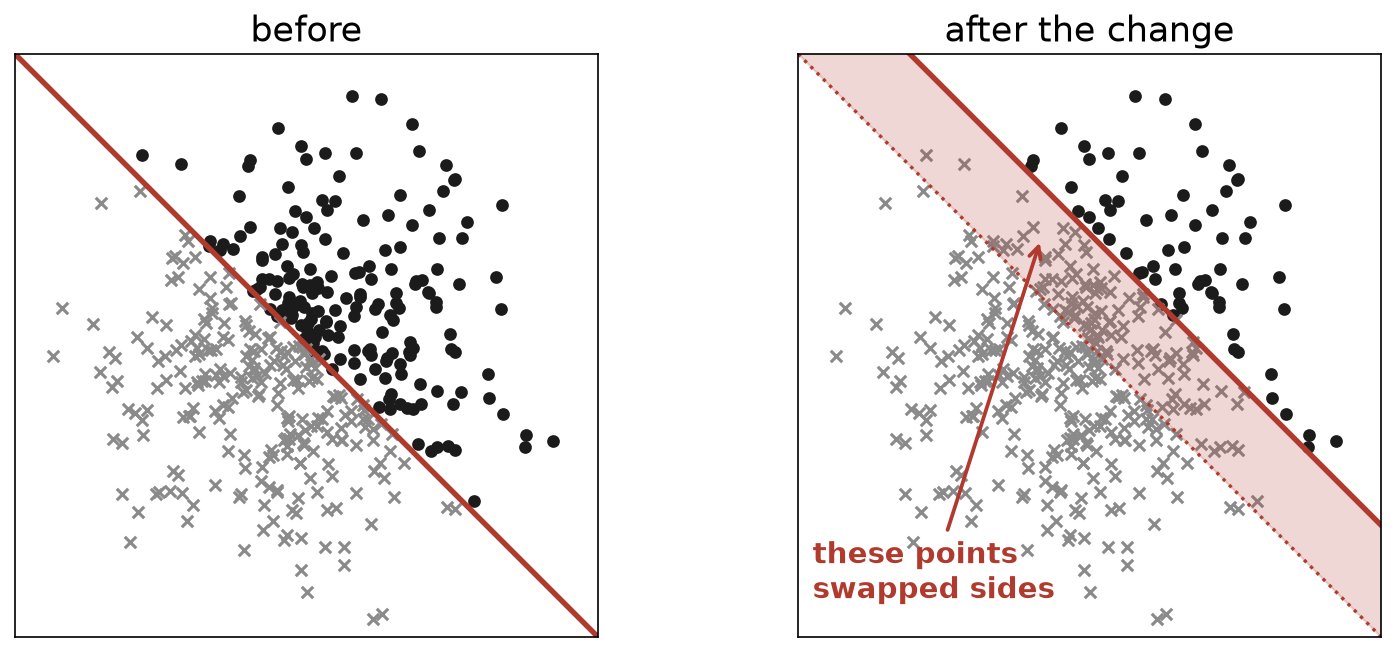
\includegraphics[height=0.60\textheight]{Fig_slide_drift.png}
  \end{center}
  \begin{center}
    A model trained on the left keeps predicting, confidently, and is now
    \alert{wrong on the shaded band}.
  \end{center}
  \note{First, the phenomenon. A model learns a rule: this input goes with
    that answer. Then the world changes and the rule no longer holds. That
    is concept drift, and here is the cleanest version of it, the one we
    simulate. Two inputs, a straight boundary, a label on each side. The
    change moves the boundary, and nothing else. Only the shaded band has
    swapped sides, and a model trained before is now wrong on it.}
\end{frame}

% ---------------------------------------------------------------- 33 s
\begin{frame}{Defence one: a model that repairs itself}
  \begin{center}
    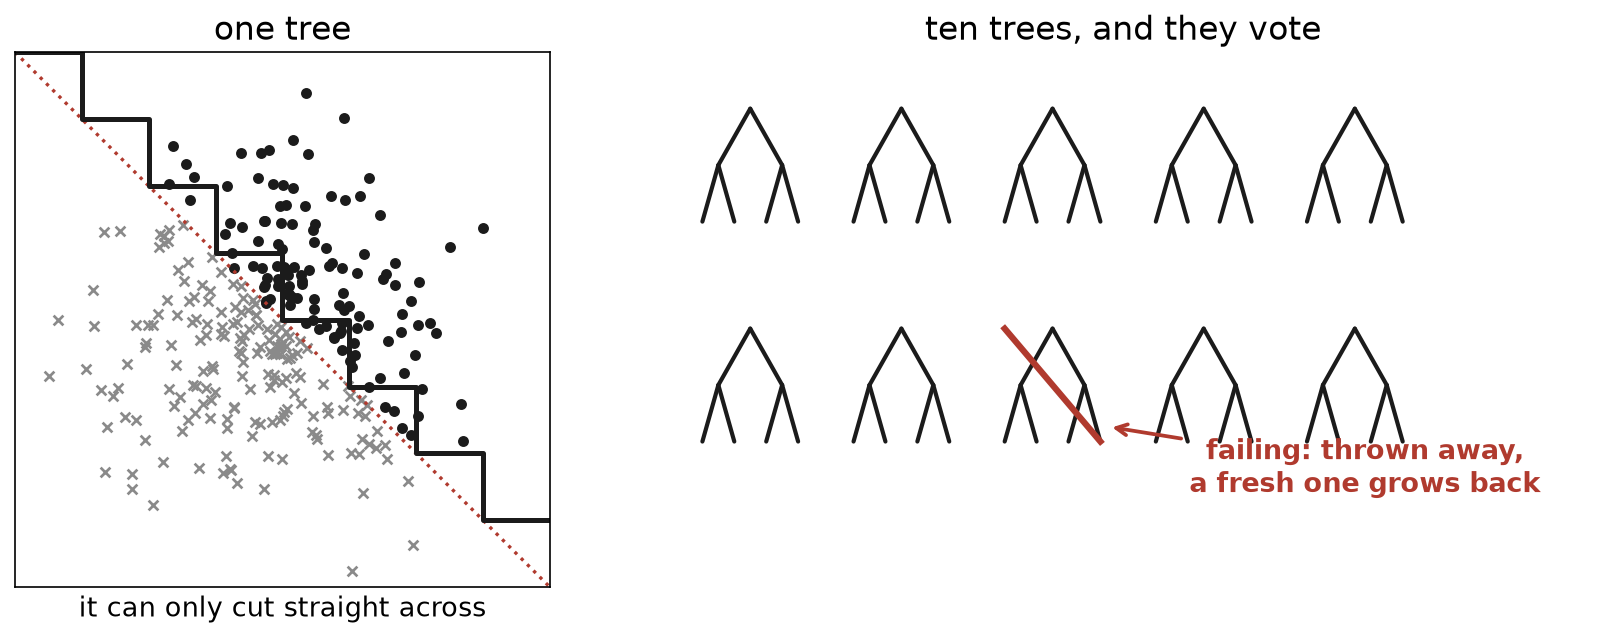
\includegraphics[width=0.94\textwidth]{Fig_slide_foret.png}
  \end{center}
  \vspace{-0.2em}
  \begin{center}
    This is the \alert{Adaptive Random Forest}. Ten trees, replaced one at a
    time.
  \end{center}
  \note{The first defence repairs itself. Its building block is a decision
    tree: it cuts the picture straight across, so a slanted boundary can
    only be approximated by a staircase. One tree is fragile, so ten of them
    vote. That is the Adaptive Random Forest, the model we study. A tree
    whose answers go wrong is thrown away, and a fresh one grows in its
    place. Ten trees, replaced one at a time.}
\end{frame}

% ---------------------------------------------------------------- 25 s
\begin{frame}{Defence two: a watchdog that raises the alarm}
  \begin{center}
    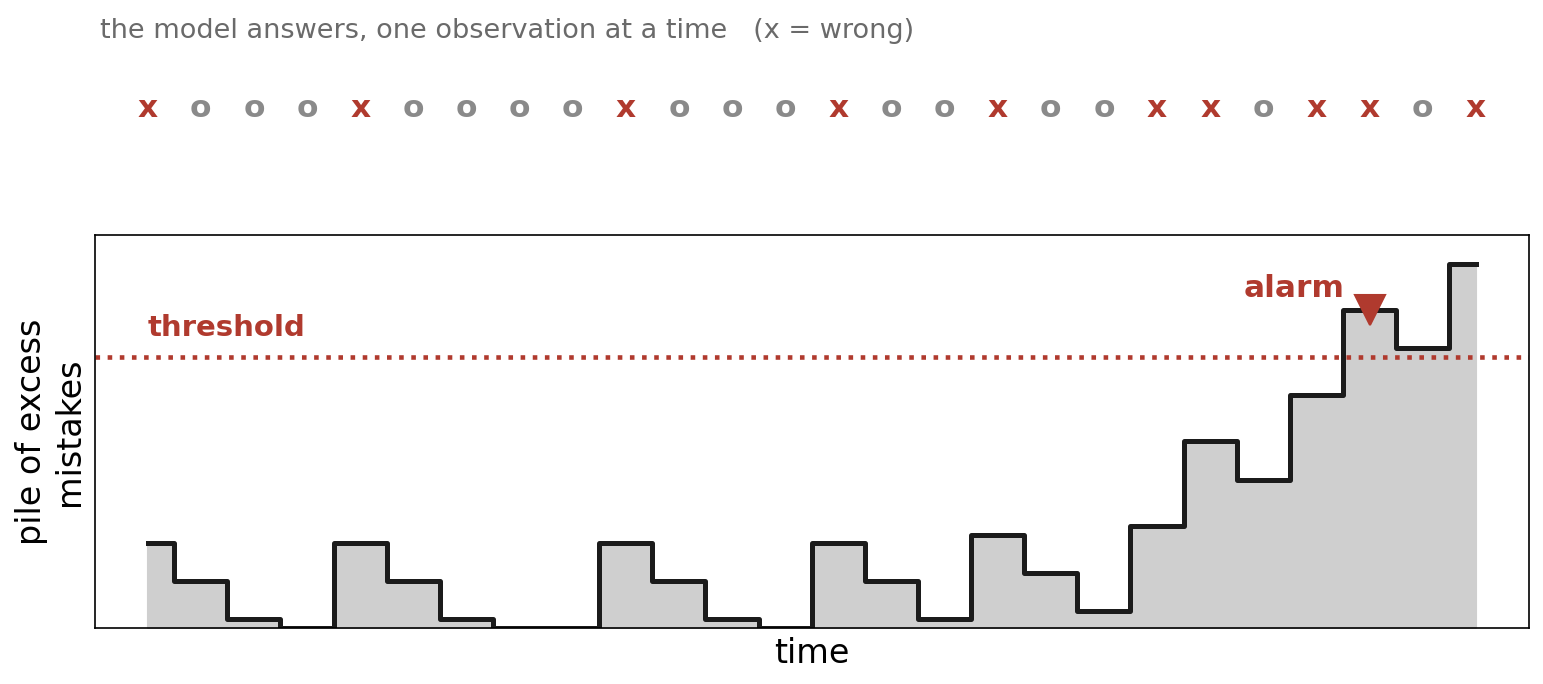
\includegraphics[width=0.94\textwidth]{Fig_slide_watchdog.png}
  \end{center}
  \vspace{-0.2em}
  \begin{center}
    Two communities, two tools, \alert{never measured against each other}.
  \end{center}
  \note{The second defence comes from a different community. A watchdog
    keeps a pile of the model's excess mistakes. While the model does well
    the pile falls back to zero; let the mistakes come and it grows, until
    it crosses a threshold and calls a human. That alarm is the only thing a
    human ever sees. Two communities, two tools, never measured against each
    other.}
\end{frame}

% ---------------------------------------------------------------- 35 s
\begin{frame}{Put them together, and they cancel out}
  \begin{center}
    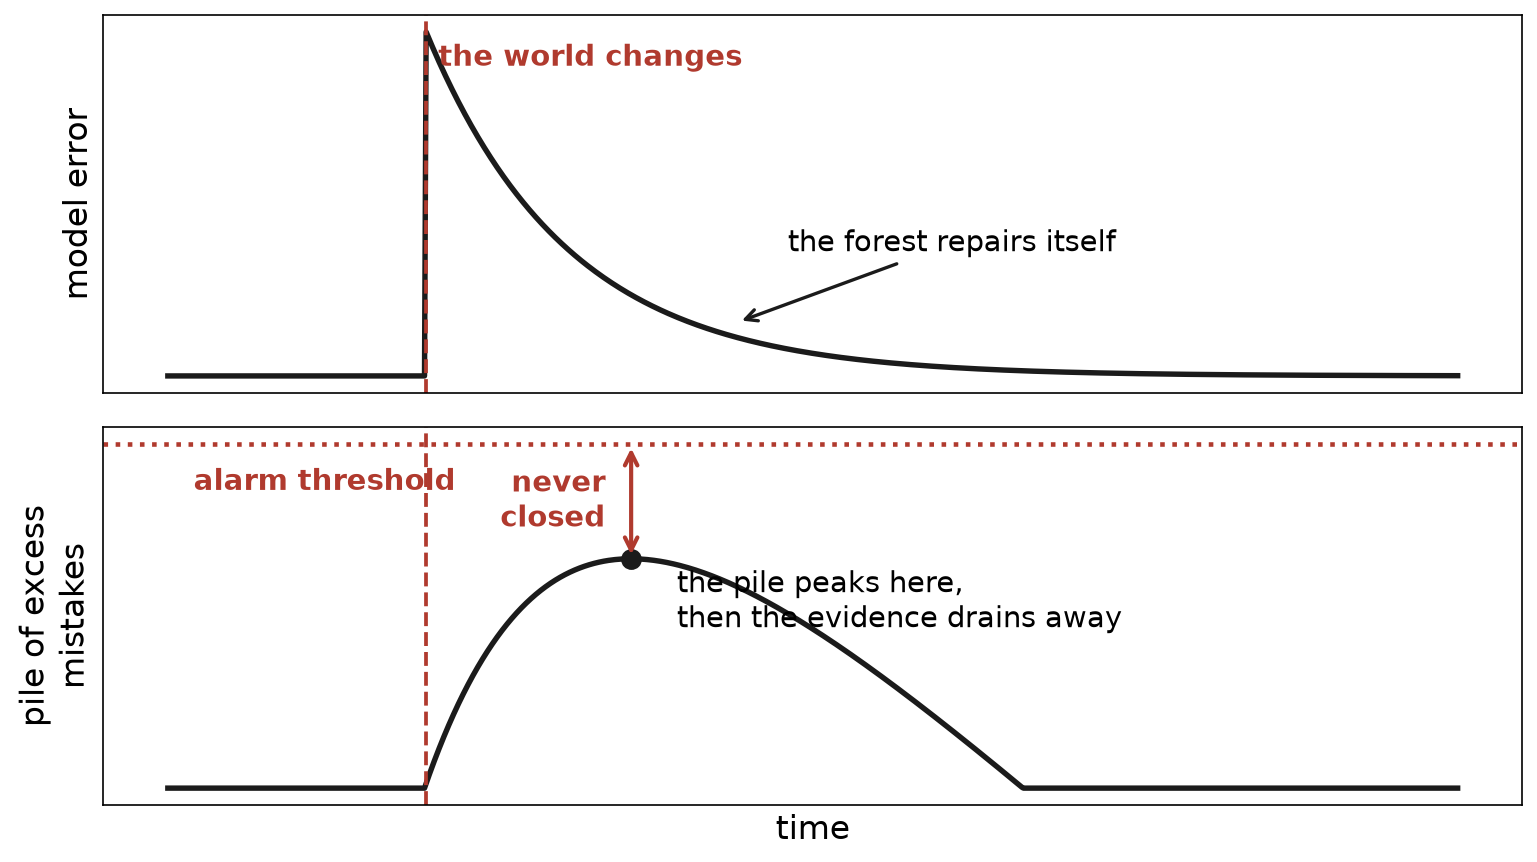
\includegraphics[height=0.70\textheight]{Fig_slide_mecanisme.png}
  \end{center}
  \vspace{-0.4em}
  \begin{center}
    \small schematic
  \end{center}
  \note{Put the two together, and they cancel out. The boundary moves, the
    mistakes begin, and the pile starts climbing. But the forest repairs
    itself, the mistakes stop, and the pile drains back to zero without ever
    reaching the threshold. The repair erased the evidence. The better the
    model fixes itself, the more surely the alarm stays silent.}
\end{frame}

% ---------------------------------------------------------------- 34 s
\begin{frame}{Why not just lower the threshold?}
  \begin{center}
    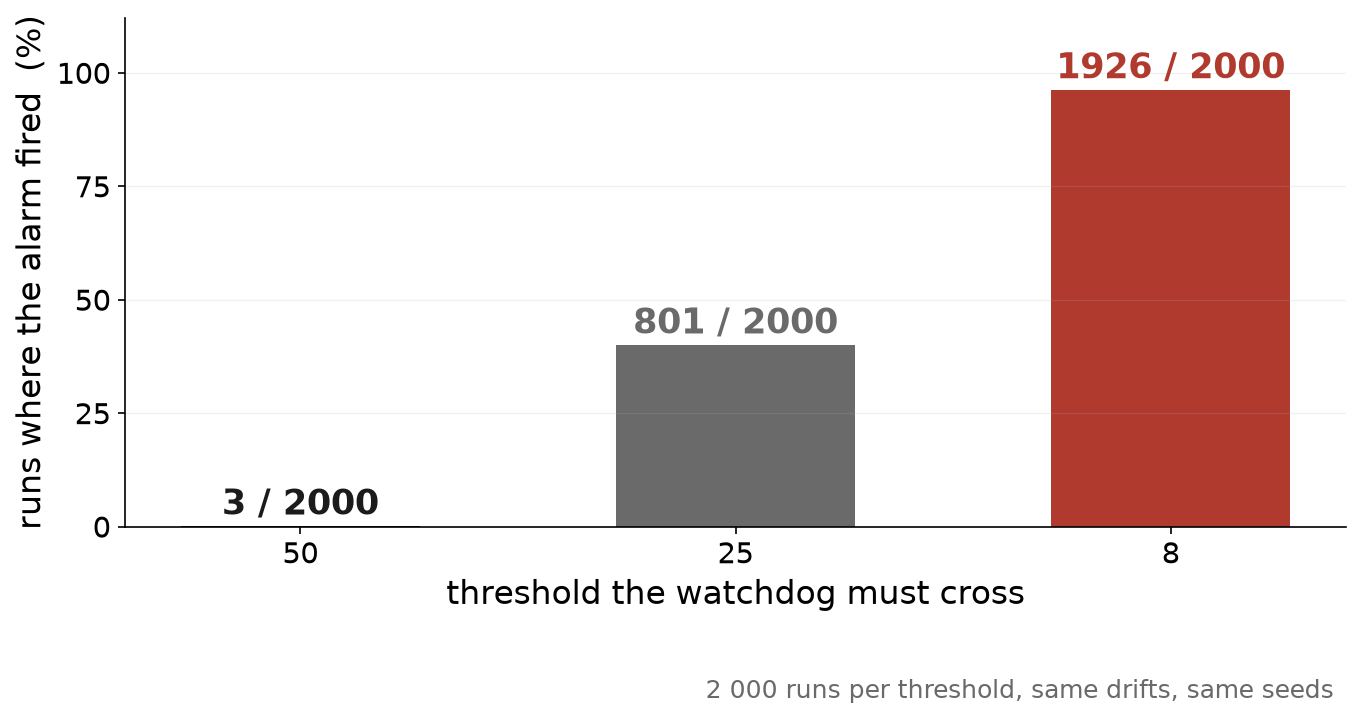
\includegraphics[width=0.80\textwidth]{Fig_slide_seuils.png}
  \end{center}
  \vspace{-0.3em}
  \begin{center}
    A low threshold also fires when \alert{nothing has happened}, and an
    alarm that cries wolf gets switched off.
  \end{center}
  \note{Does the alarm ever fire? That depends on the threshold. We re-ran
    the benchmark at three settings, two thousand runs each. At the highest
    it fired three times out of two thousand. Lower it, and it fires almost
    every time. So why not lower it? Because a low threshold also fires when
    nothing happened, and an alarm that cries wolf gets switched off. The
    setting quiet enough to be trusted is the one that never sees the
    drift.}
\end{frame}

% ---------------------------------------------------------------- 33 s
\begin{frame}{Our contribution: when is the forest actually repaired?}
  \begin{center}
    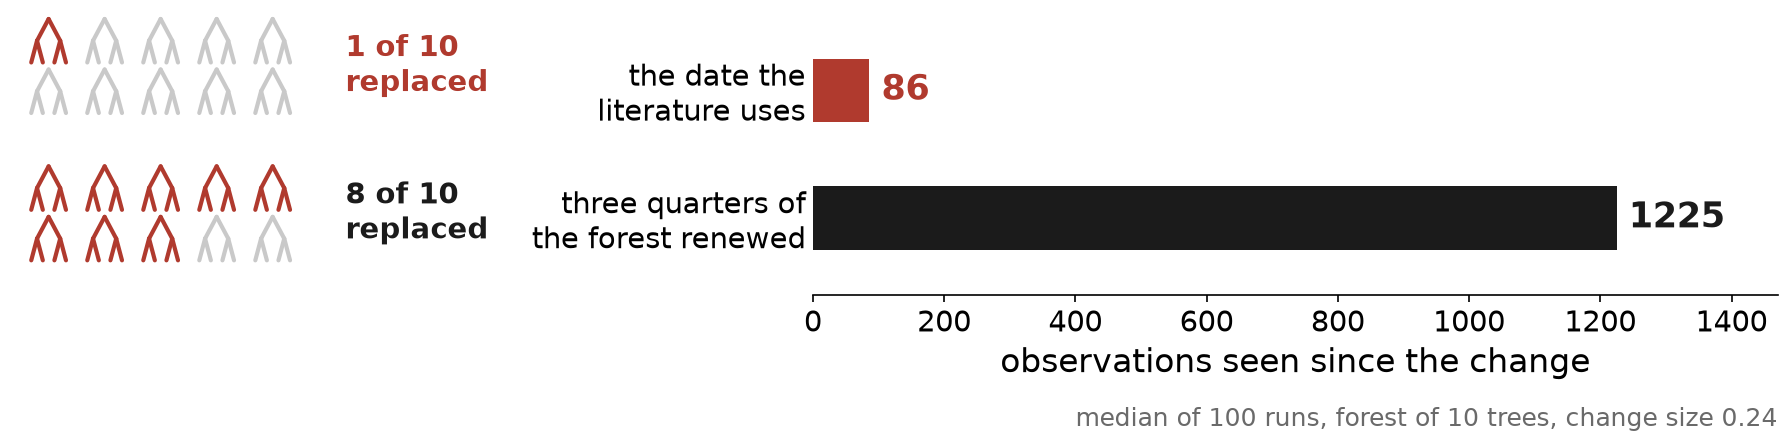
\includegraphics[width=\textwidth]{Fig_slide_deux_horloges.png}
  \end{center}
  \vspace{0.1em}
  \begin{center}
    \alert{\large The accepted date fires at the \emph{first} tree. It times
    the start of a repair, not its end.}
  \end{center}
  \note{It is a race, so we have to time both runners. Timing the alarm is
    easy. Timing the repair is where we found something. The literature has
    a standard date for it, and that date turns out to be the moment the
    very first tree out of ten is replaced. Wait until three quarters of the
    forest has actually been renewed, and you wait roughly ten times longer.
    That stopwatch times the start of a repair, not its end, and it is wrong
    always in the same direction.}
\end{frame}

% ---------------------------------------------------------------- 22 s
\begin{frame}{Where we stand}
  \begin{itemize}
    \item The paradox is \alert{real and reproducible}, and we can say when
          the evidence falls short of what the alarm needs.
    \item The clock the field relies on is \alert{biased, always the same
          way}. Every conclusion drawn from it inherits that bias.
    \item \textbf{Next}: watch the model and the watchdog on one common
          clock, and turn this into advice a practitioner can use.
  \end{itemize}
  \vfill
  \begin{center}
    \large Thank you.
  \end{center}
  \note{Where we stand. The paradox is real and reproducible. The clock the
    field relies on is biased, always the same way, so every conclusion
    drawn from it inherits that bias. What remains is to turn this into
    advice a practitioner can use. Thank you.}
\end{frame}

\end{document}
"
\ifdefined\NOTESSEULES\setbeameroption{show only notes}\fi
\graphicspath{{../04_experimentations/resultats_R2/resultats/figures/}}

% Fontes resserrees pour que les quatre auteurs tiennent sur une ligne.
% (L'« Overfull vbox » de la page de titre vient du theme metropolis
% lui-meme : il se reproduit a l'identique avec un titre d'un seul
% caractere, et rien n'est coupe au rendu. Ne pas chercher a le corriger.)
\setbeamerfont{author}{size=\small}
\setbeamerfont{institute}{size=\scriptsize}

\title{The Blind Spot Paradox}
\subtitle{When a self-repairing model destroys the evidence its own monitor needs}
\author{Alexandre Boyer \and Mélaine Gouillou \and Salomé Fonvielle \and Ulysse Petit-Tichanné}
\institute{Research Track, Topic 39, CentraleSupélec. Supervisor: Raphaël Minato}
\date{}

\begin{document}

\maketitle
\note{The Blind Spot Paradox: when a self-repairing model destroys the
  evidence its own monitor needs.}

% ---------------------------------------------------------------- 32 s
\begin{frame}{Concept drift: the rule changes, the data does not}
  \begin{center}
    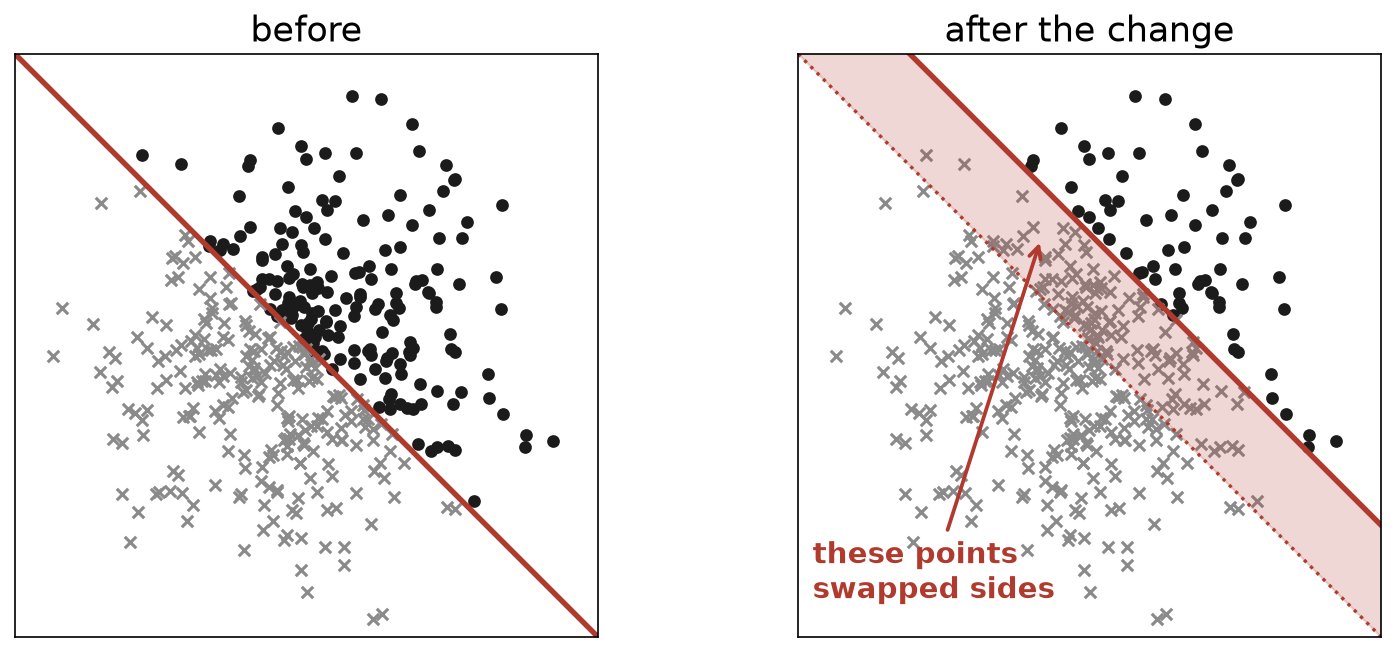
\includegraphics[height=0.60\textheight]{Fig_slide_drift.png}
  \end{center}
  \begin{center}
    A model trained on the left keeps predicting, confidently, and is now
    \alert{wrong on the shaded band}.
  \end{center}
  \note{First, the phenomenon. A model learns a rule: this input goes with
    that answer. Then the world changes and the rule no longer holds. That
    is concept drift, and here is the cleanest version of it, the one we
    simulate. Two inputs, a straight boundary, a label on each side. The
    change moves the boundary, and nothing else. Only the shaded band has
    swapped sides, and a model trained before is now wrong on it.}
\end{frame}

% ---------------------------------------------------------------- 33 s
\begin{frame}{Defence one: a model that repairs itself}
  \begin{center}
    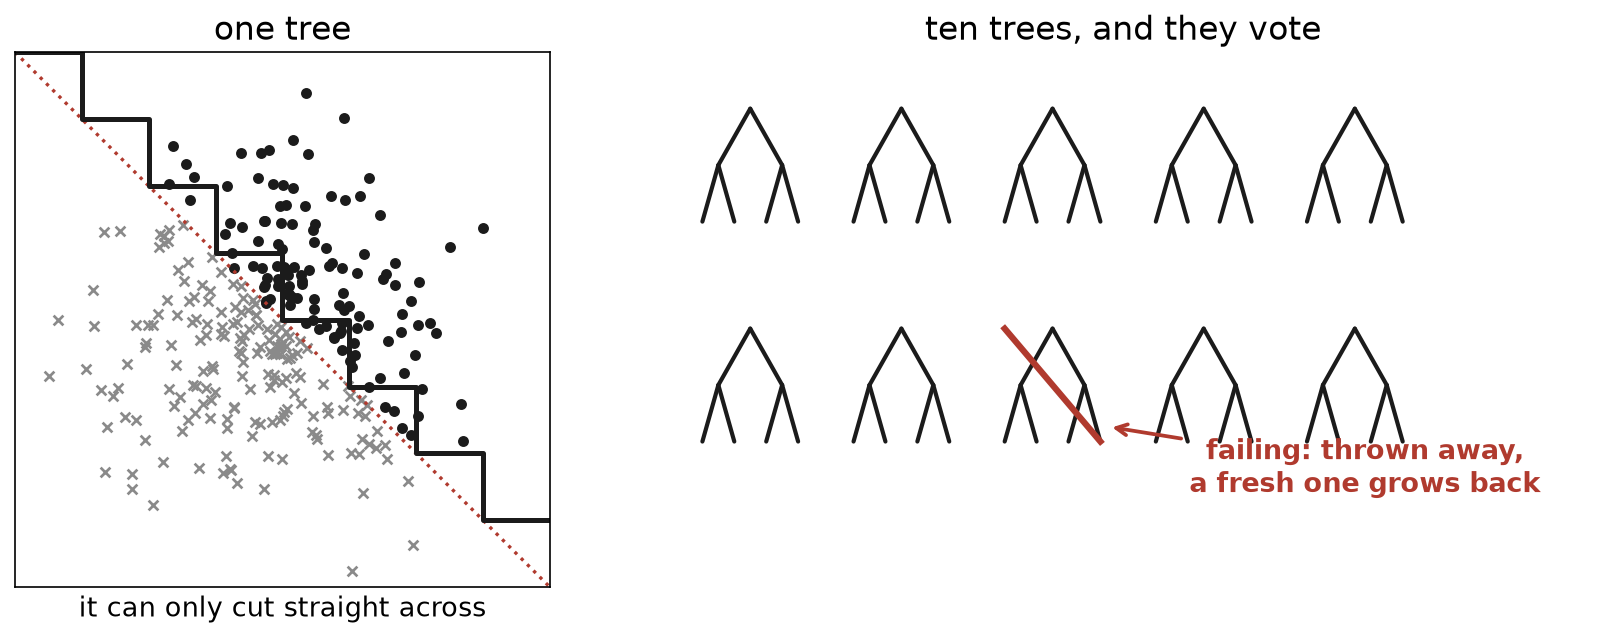
\includegraphics[width=0.94\textwidth]{Fig_slide_foret.png}
  \end{center}
  \vspace{-0.2em}
  \begin{center}
    This is the \alert{Adaptive Random Forest}. Ten trees, replaced one at a
    time.
  \end{center}
  \note{The first defence repairs itself. Its building block is a decision
    tree: it cuts the picture straight across, so a slanted boundary can
    only be approximated by a staircase. One tree is fragile, so ten of them
    vote. That is the Adaptive Random Forest, the model we study. A tree
    whose answers go wrong is thrown away, and a fresh one grows in its
    place. Ten trees, replaced one at a time.}
\end{frame}

% ---------------------------------------------------------------- 25 s
\begin{frame}{Defence two: a watchdog that raises the alarm}
  \begin{center}
    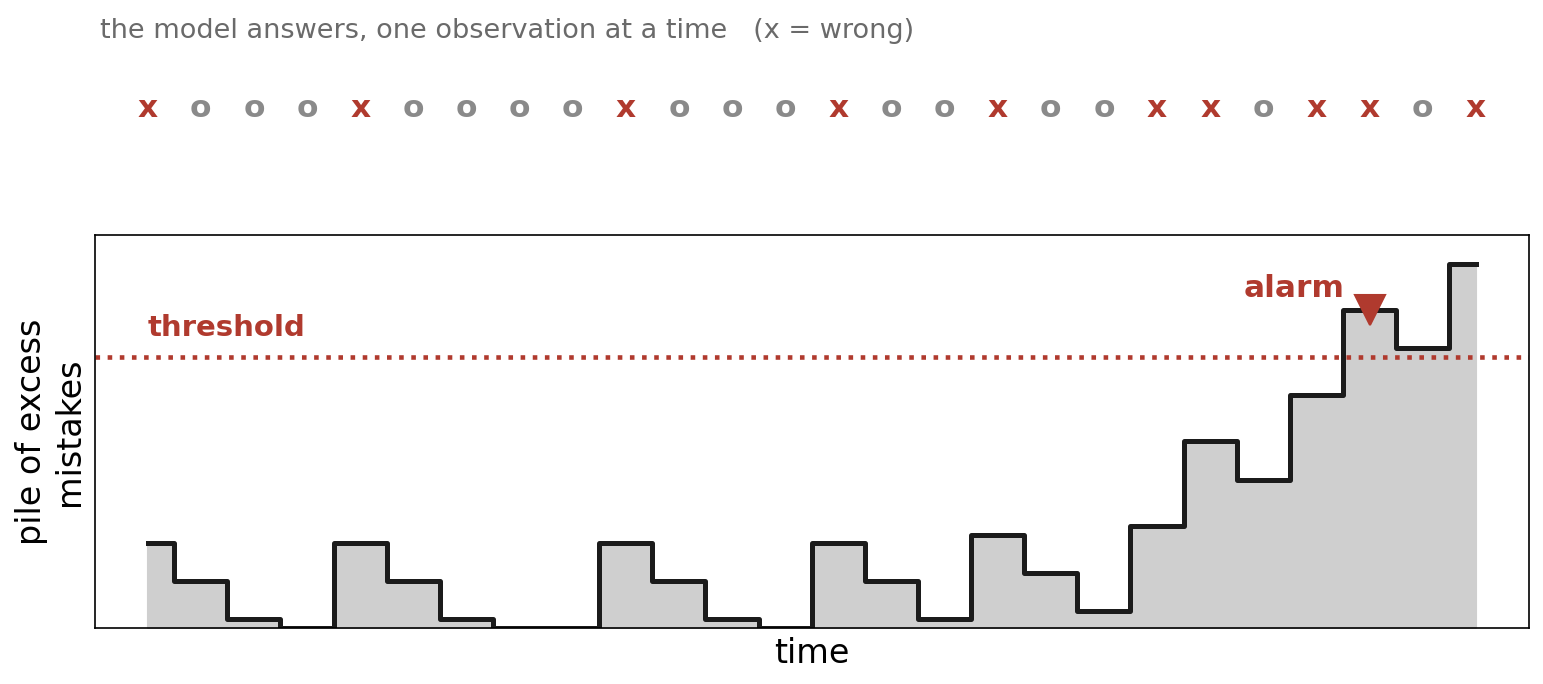
\includegraphics[width=0.94\textwidth]{Fig_slide_watchdog.png}
  \end{center}
  \vspace{-0.2em}
  \begin{center}
    Two communities, two tools, \alert{never measured against each other}.
  \end{center}
  \note{The second defence comes from a different community. A watchdog
    keeps a pile of the model's excess mistakes. While the model does well
    the pile falls back to zero; let the mistakes come and it grows, until
    it crosses a threshold and calls a human. That alarm is the only thing a
    human ever sees. Two communities, two tools, never measured against each
    other.}
\end{frame}

% ---------------------------------------------------------------- 35 s
\begin{frame}{Put them together, and they cancel out}
  \begin{center}
    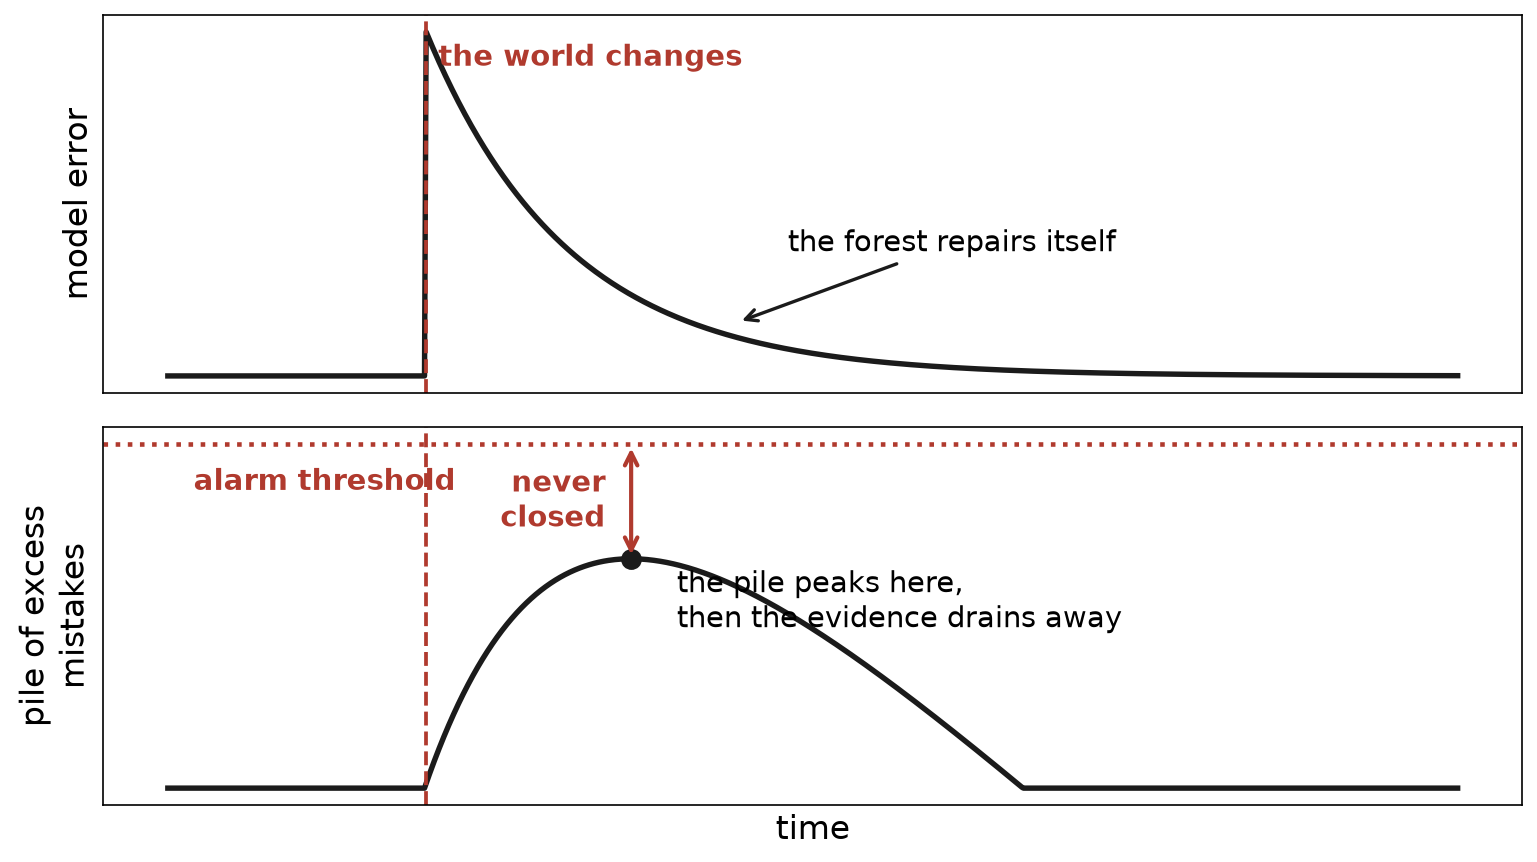
\includegraphics[height=0.70\textheight]{Fig_slide_mecanisme.png}
  \end{center}
  \vspace{-0.4em}
  \begin{center}
    \small schematic
  \end{center}
  \note{Put the two together, and they cancel out. The boundary moves, the
    mistakes begin, and the pile starts climbing. But the forest repairs
    itself, the mistakes stop, and the pile drains back to zero without ever
    reaching the threshold. The repair erased the evidence. The better the
    model fixes itself, the more surely the alarm stays silent.}
\end{frame}

% ---------------------------------------------------------------- 34 s
\begin{frame}{Why not just lower the threshold?}
  \begin{center}
    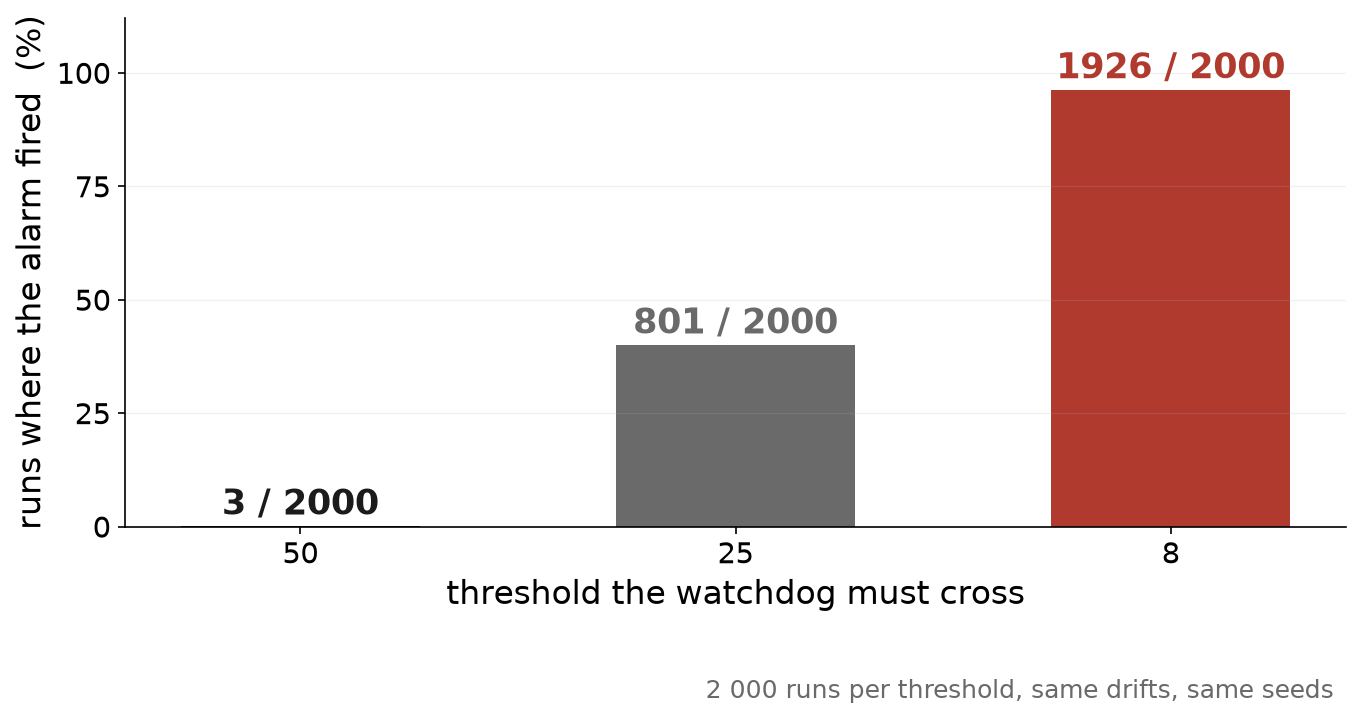
\includegraphics[width=0.80\textwidth]{Fig_slide_seuils.png}
  \end{center}
  \vspace{-0.3em}
  \begin{center}
    A low threshold also fires when \alert{nothing has happened}, and an
    alarm that cries wolf gets switched off.
  \end{center}
  \note{Does the alarm ever fire? That depends on the threshold. We re-ran
    the benchmark at three settings, two thousand runs each. At the highest
    it fired three times out of two thousand. Lower it, and it fires almost
    every time. So why not lower it? Because a low threshold also fires when
    nothing happened, and an alarm that cries wolf gets switched off. The
    setting quiet enough to be trusted is the one that never sees the
    drift.}
\end{frame}

% ---------------------------------------------------------------- 33 s
\begin{frame}{Our contribution: when is the forest actually repaired?}
  \begin{center}
    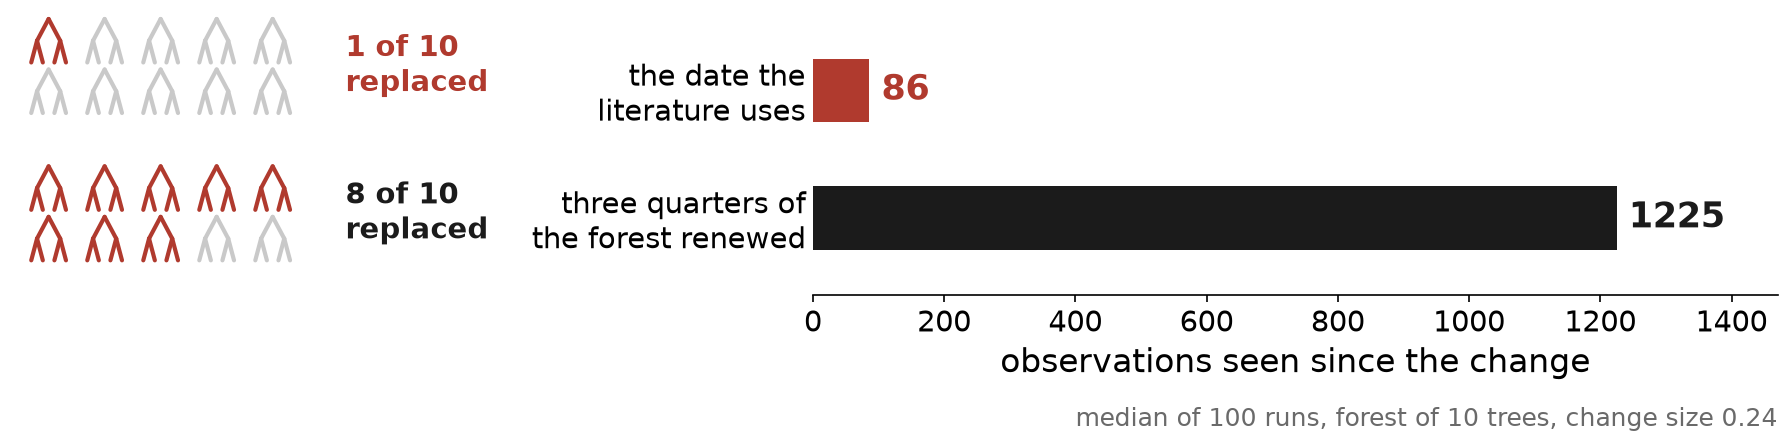
\includegraphics[width=\textwidth]{Fig_slide_deux_horloges.png}
  \end{center}
  \vspace{0.1em}
  \begin{center}
    \alert{\large The accepted date fires at the \emph{first} tree. It times
    the start of a repair, not its end.}
  \end{center}
  \note{It is a race, so we have to time both runners. Timing the alarm is
    easy. Timing the repair is where we found something. The literature has
    a standard date for it, and that date turns out to be the moment the
    very first tree out of ten is replaced. Wait until three quarters of the
    forest has actually been renewed, and you wait roughly ten times longer.
    That stopwatch times the start of a repair, not its end, and it is wrong
    always in the same direction.}
\end{frame}

% ---------------------------------------------------------------- 22 s
\begin{frame}{Where we stand}
  \begin{itemize}
    \item The paradox is \alert{real and reproducible}, and we can say when
          the evidence falls short of what the alarm needs.
    \item The clock the field relies on is \alert{biased, always the same
          way}. Every conclusion drawn from it inherits that bias.
    \item \textbf{Next}: watch the model and the watchdog on one common
          clock, and turn this into advice a practitioner can use.
  \end{itemize}
  \vfill
  \begin{center}
    \large Thank you.
  \end{center}
  \note{Where we stand. The paradox is real and reproducible. The clock the
    field relies on is biased, always the same way, so every conclusion
    drawn from it inherits that bias. What remains is to turn this into
    advice a practitioner can use. Thank you.}
\end{frame}

\end{document}
"
\ifdefined\NOTESSEULES\setbeameroption{show only notes}\fi
\graphicspath{{../04_experimentations/resultats_R2/resultats/figures/}}

% Fontes resserrees pour que les quatre auteurs tiennent sur une ligne.
% (L'« Overfull vbox » de la page de titre vient du theme metropolis
% lui-meme : il se reproduit a l'identique avec un titre d'un seul
% caractere, et rien n'est coupe au rendu. Ne pas chercher a le corriger.)
\setbeamerfont{author}{size=\small}
\setbeamerfont{institute}{size=\scriptsize}

\title{The Blind Spot Paradox}
\subtitle{When a self-repairing model destroys the evidence its own monitor needs}
\author{Alexandre Boyer \and Mélaine Gouillou \and Salomé Fonvielle \and Ulysse Petit-Tichanné}
\institute{Research Track, Topic 39, CentraleSupélec. Supervisor: Raphaël Minato}
\date{}

\begin{document}

\maketitle
\note{The Blind Spot Paradox: when a self-repairing model destroys the
  evidence its own monitor needs.}

% ---------------------------------------------------------------- 32 s
\begin{frame}{Concept drift: the rule changes, the data does not}
  \begin{center}
    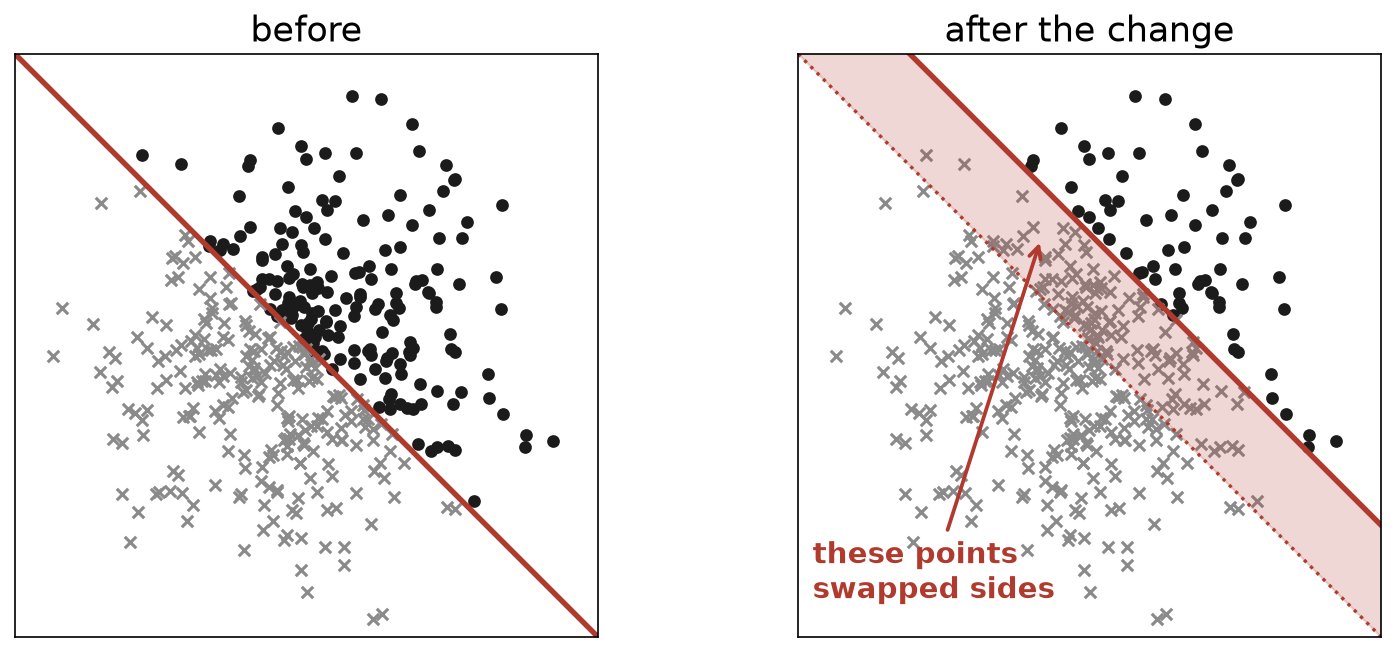
\includegraphics[height=0.60\textheight]{Fig_slide_drift.png}
  \end{center}
  \begin{center}
    A model trained on the left keeps predicting, confidently, and is now
    \alert{wrong on the shaded band}.
  \end{center}
  \note{First, the phenomenon. A model learns a rule: this input goes with
    that answer. Then the world changes and the rule no longer holds. That
    is concept drift, and here is the cleanest version of it, the one we
    simulate. Two inputs, a straight boundary, a label on each side. The
    change moves the boundary, and nothing else. Only the shaded band has
    swapped sides, and a model trained before is now wrong on it.}
\end{frame}

% ---------------------------------------------------------------- 33 s
\begin{frame}{Defence one: a model that repairs itself}
  \begin{center}
    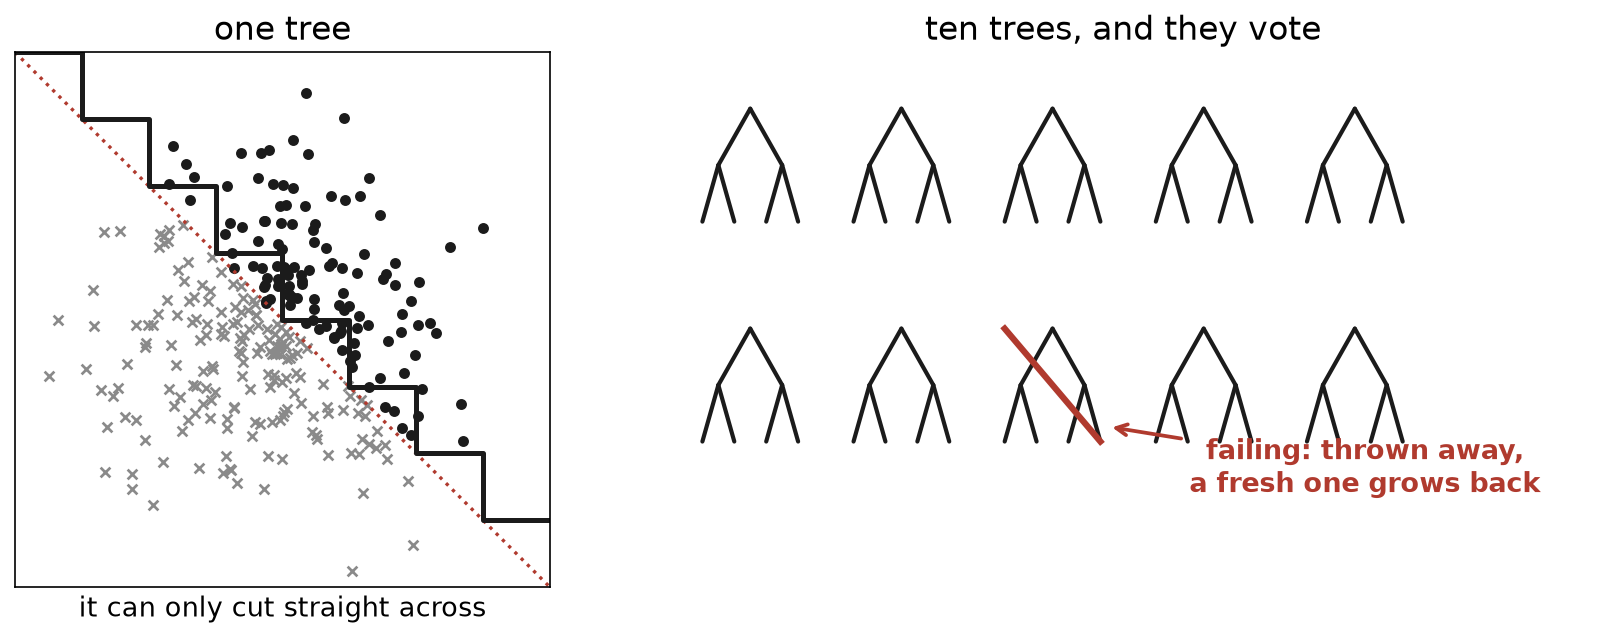
\includegraphics[width=0.94\textwidth]{Fig_slide_foret.png}
  \end{center}
  \vspace{-0.2em}
  \begin{center}
    This is the \alert{Adaptive Random Forest}. Ten trees, replaced one at a
    time.
  \end{center}
  \note{The first defence repairs itself. Its building block is a decision
    tree: it cuts the picture straight across, so a slanted boundary can
    only be approximated by a staircase. One tree is fragile, so ten of them
    vote. That is the Adaptive Random Forest, the model we study. A tree
    whose answers go wrong is thrown away, and a fresh one grows in its
    place. Ten trees, replaced one at a time.}
\end{frame}

% ---------------------------------------------------------------- 25 s
\begin{frame}{Defence two: a watchdog that raises the alarm}
  \begin{center}
    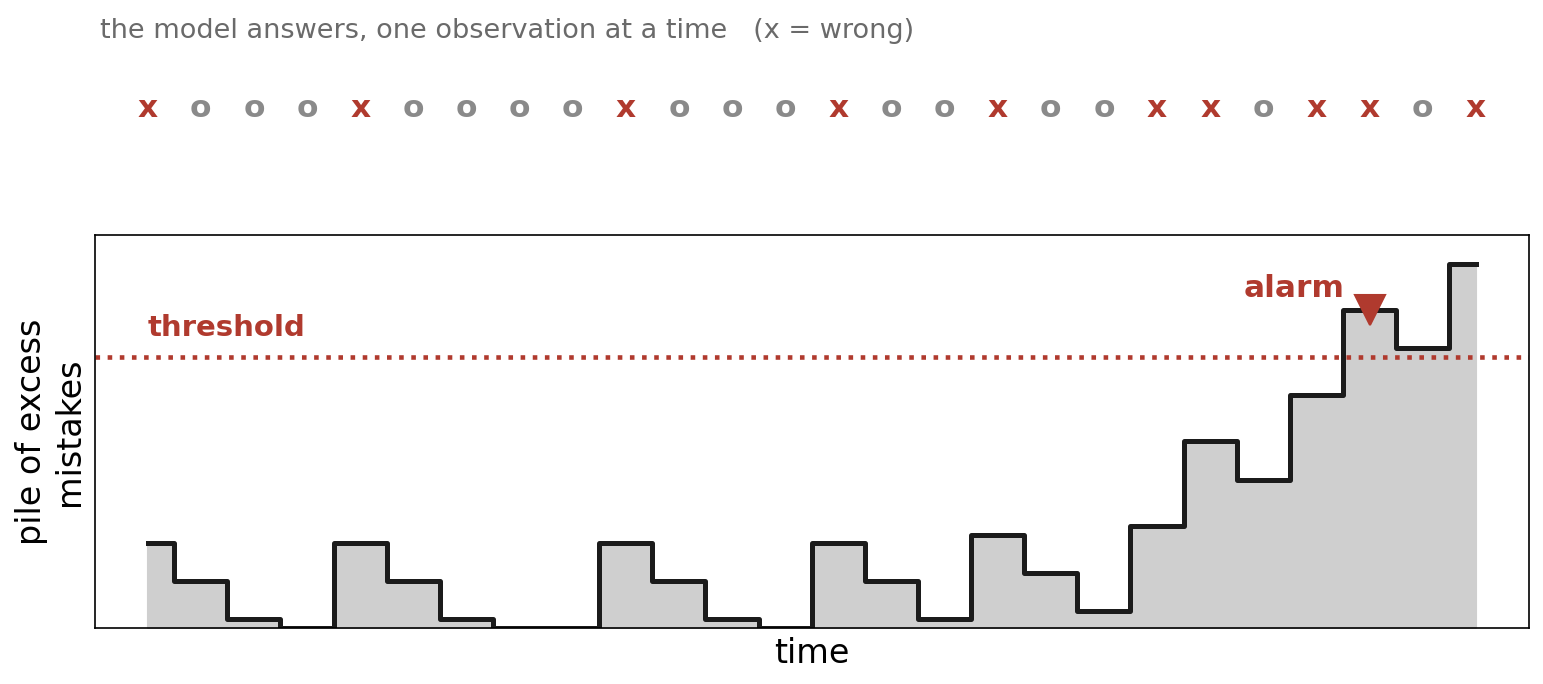
\includegraphics[width=0.94\textwidth]{Fig_slide_watchdog.png}
  \end{center}
  \vspace{-0.2em}
  \begin{center}
    Two communities, two tools, \alert{never measured against each other}.
  \end{center}
  \note{The second defence comes from a different community. A watchdog
    keeps a pile of the model's excess mistakes. While the model does well
    the pile falls back to zero; let the mistakes come and it grows, until
    it crosses a threshold and calls a human. That alarm is the only thing a
    human ever sees. Two communities, two tools, never measured against each
    other.}
\end{frame}

% ---------------------------------------------------------------- 35 s
\begin{frame}{Put them together, and they cancel out}
  \begin{center}
    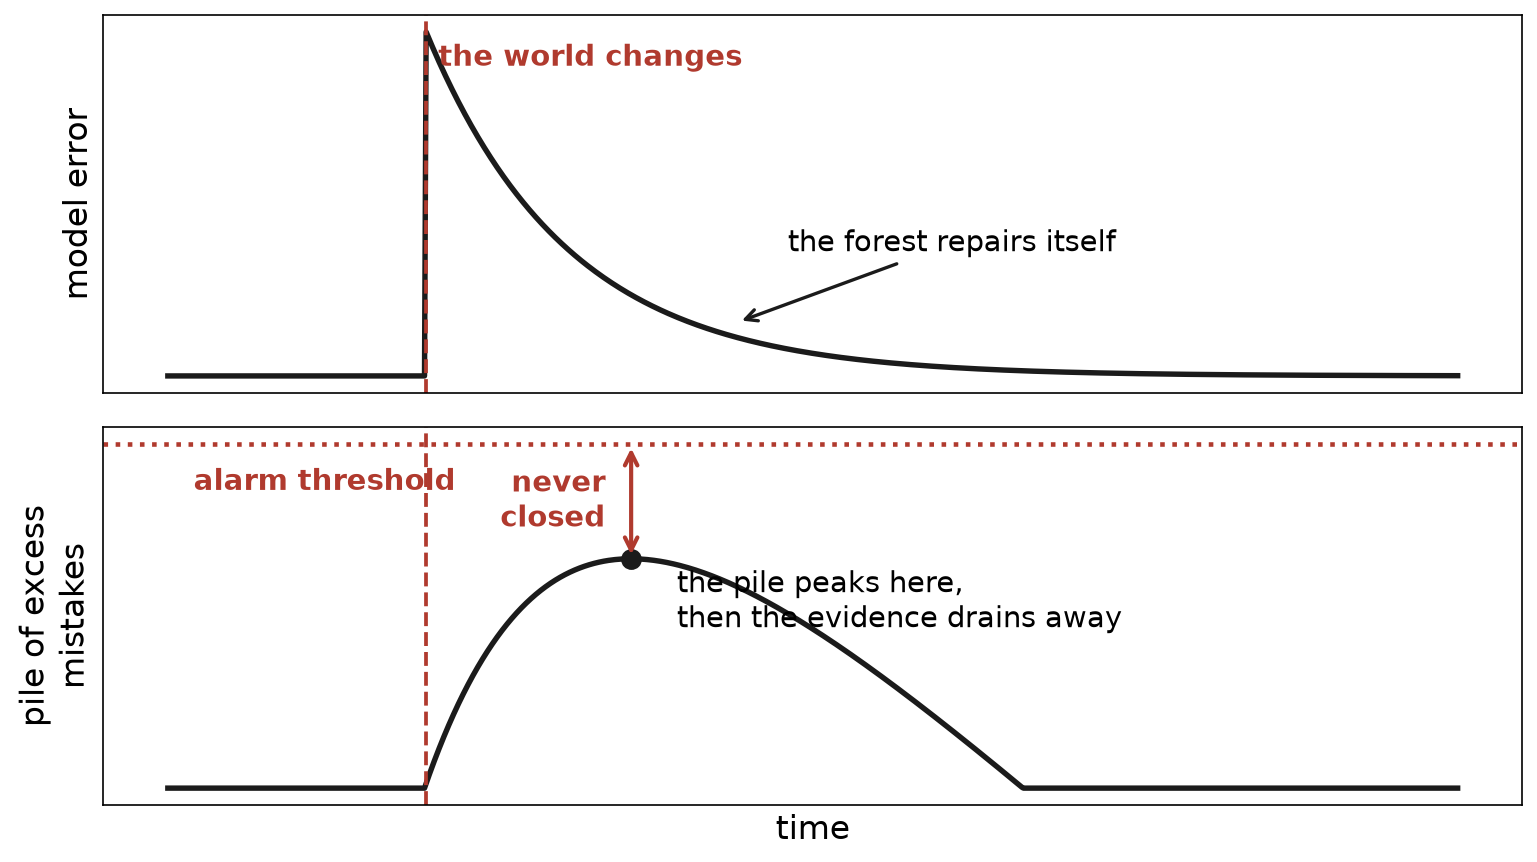
\includegraphics[height=0.70\textheight]{Fig_slide_mecanisme.png}
  \end{center}
  \vspace{-0.4em}
  \begin{center}
    \small schematic
  \end{center}
  \note{Put the two together, and they cancel out. The boundary moves, the
    mistakes begin, and the pile starts climbing. But the forest repairs
    itself, the mistakes stop, and the pile drains back to zero without ever
    reaching the threshold. The repair erased the evidence. The better the
    model fixes itself, the more surely the alarm stays silent.}
\end{frame}

% ---------------------------------------------------------------- 34 s
\begin{frame}{Why not just lower the threshold?}
  \begin{center}
    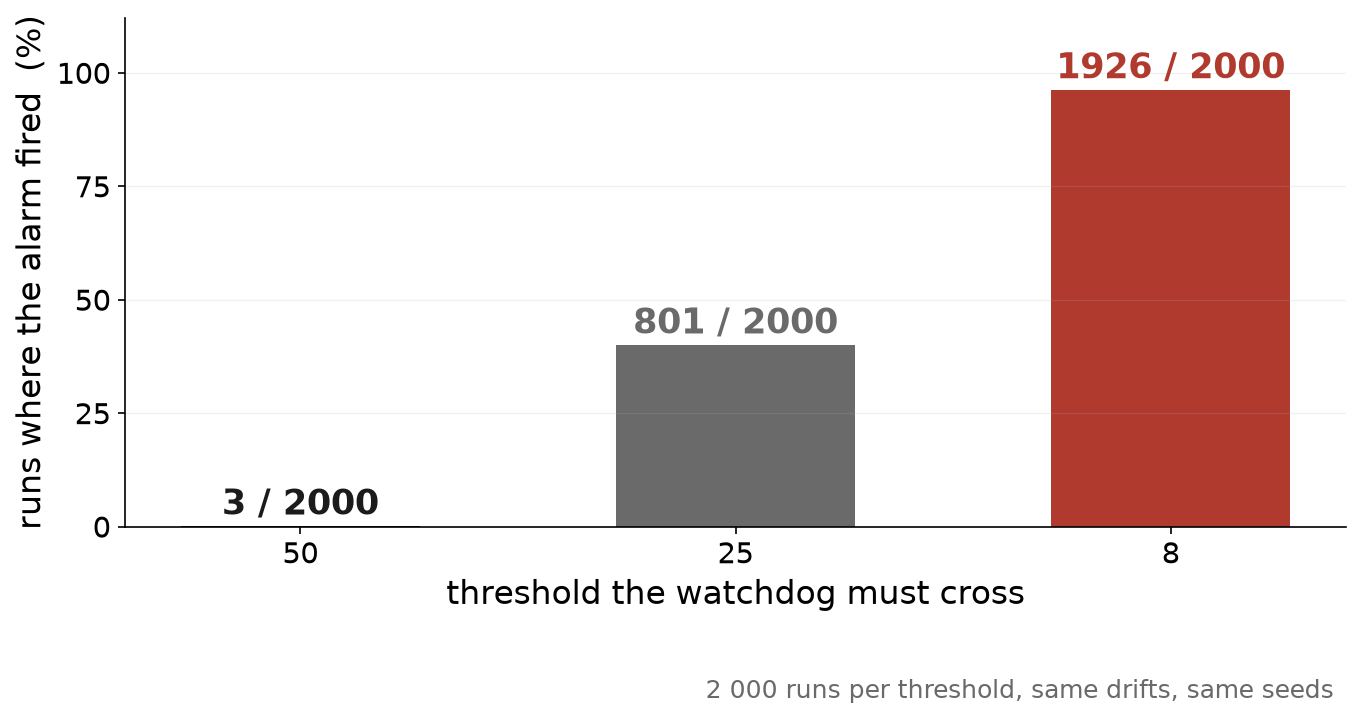
\includegraphics[width=0.80\textwidth]{Fig_slide_seuils.png}
  \end{center}
  \vspace{-0.3em}
  \begin{center}
    A low threshold also fires when \alert{nothing has happened}, and an
    alarm that cries wolf gets switched off.
  \end{center}
  \note{Does the alarm ever fire? That depends on the threshold. We re-ran
    the benchmark at three settings, two thousand runs each. At the highest
    it fired three times out of two thousand. Lower it, and it fires almost
    every time. So why not lower it? Because a low threshold also fires when
    nothing happened, and an alarm that cries wolf gets switched off. The
    setting quiet enough to be trusted is the one that never sees the
    drift.}
\end{frame}

% ---------------------------------------------------------------- 33 s
\begin{frame}{Our contribution: when is the forest actually repaired?}
  \begin{center}
    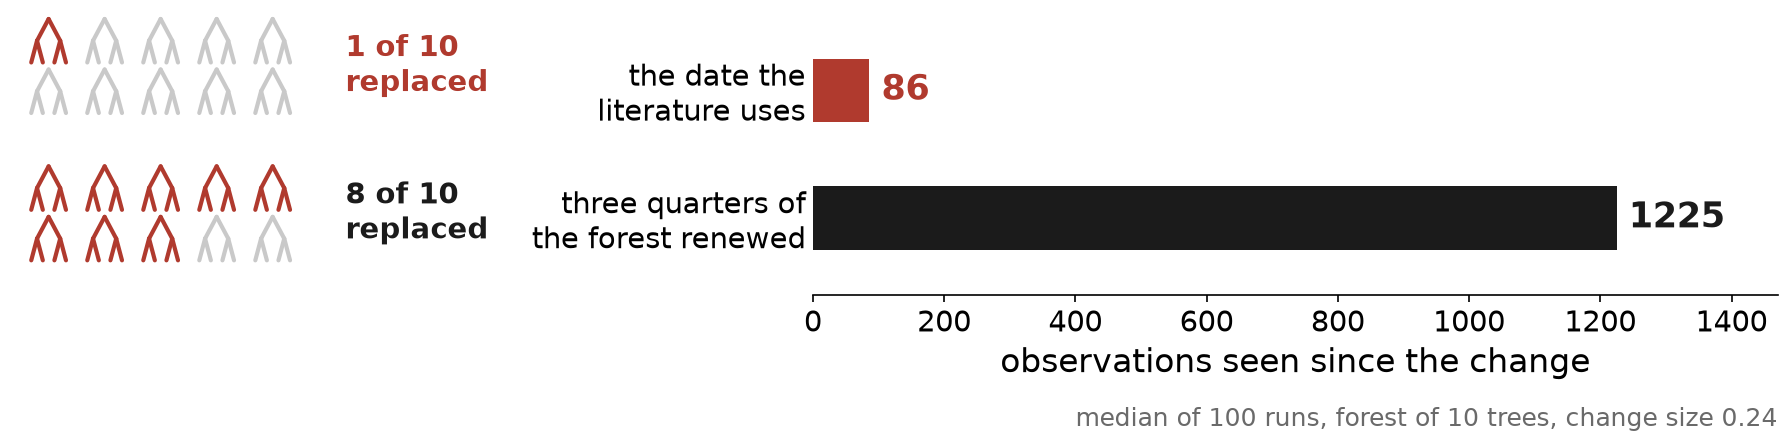
\includegraphics[width=\textwidth]{Fig_slide_deux_horloges.png}
  \end{center}
  \vspace{0.1em}
  \begin{center}
    \alert{\large The accepted date fires at the \emph{first} tree. It times
    the start of a repair, not its end.}
  \end{center}
  \note{It is a race, so we have to time both runners. Timing the alarm is
    easy. Timing the repair is where we found something. The literature has
    a standard date for it, and that date turns out to be the moment the
    very first tree out of ten is replaced. Wait until three quarters of the
    forest has actually been renewed, and you wait roughly ten times longer.
    That stopwatch times the start of a repair, not its end, and it is wrong
    always in the same direction.}
\end{frame}

% ---------------------------------------------------------------- 22 s
\begin{frame}{Where we stand}
  \begin{itemize}
    \item The paradox is \alert{real and reproducible}, and we can say when
          the evidence falls short of what the alarm needs.
    \item The clock the field relies on is \alert{biased, always the same
          way}. Every conclusion drawn from it inherits that bias.
    \item \textbf{Next}: watch the model and the watchdog on one common
          clock, and turn this into advice a practitioner can use.
  \end{itemize}
  \vfill
  \begin{center}
    \large Thank you.
  \end{center}
  \note{Where we stand. The paradox is real and reproducible. The clock the
    field relies on is biased, always the same way, so every conclusion
    drawn from it inherits that bias. What remains is to turn this into
    advice a practitioner can use. Thank you.}
\end{frame}

\end{document}
"
\ifdefined\NOTESSEULES\setbeameroption{show only notes}\fi
\graphicspath{{../04_experimentations/resultats_R2/resultats/figures/}}

% Fontes resserrees pour que les quatre auteurs tiennent sur une ligne.
% (L'« Overfull vbox » de la page de titre vient du theme metropolis
% lui-meme : il se reproduit a l'identique avec un titre d'un seul
% caractere, et rien n'est coupe au rendu. Ne pas chercher a le corriger.)
\setbeamerfont{author}{size=\small}
\setbeamerfont{institute}{size=\scriptsize}

\title{The Blind Spot Paradox}
\subtitle{When a self-repairing model destroys the evidence its own monitor needs}
\author{Alexandre Boyer \and Mélaine Gouillou \and Salomé Fonvielle \and Ulysse Petit-Tichanné}
\institute{Research Track, Topic 39, CentraleSupélec. Supervisor: Raphaël Minato}
\date{}

\begin{document}

\maketitle
\note{The Blind Spot Paradox: when a self-repairing model destroys the
  evidence its own monitor needs.}

% ---------------------------------------------------------------- 32 s
\begin{frame}{Concept drift: the rule changes, the data does not}
  \begin{center}
    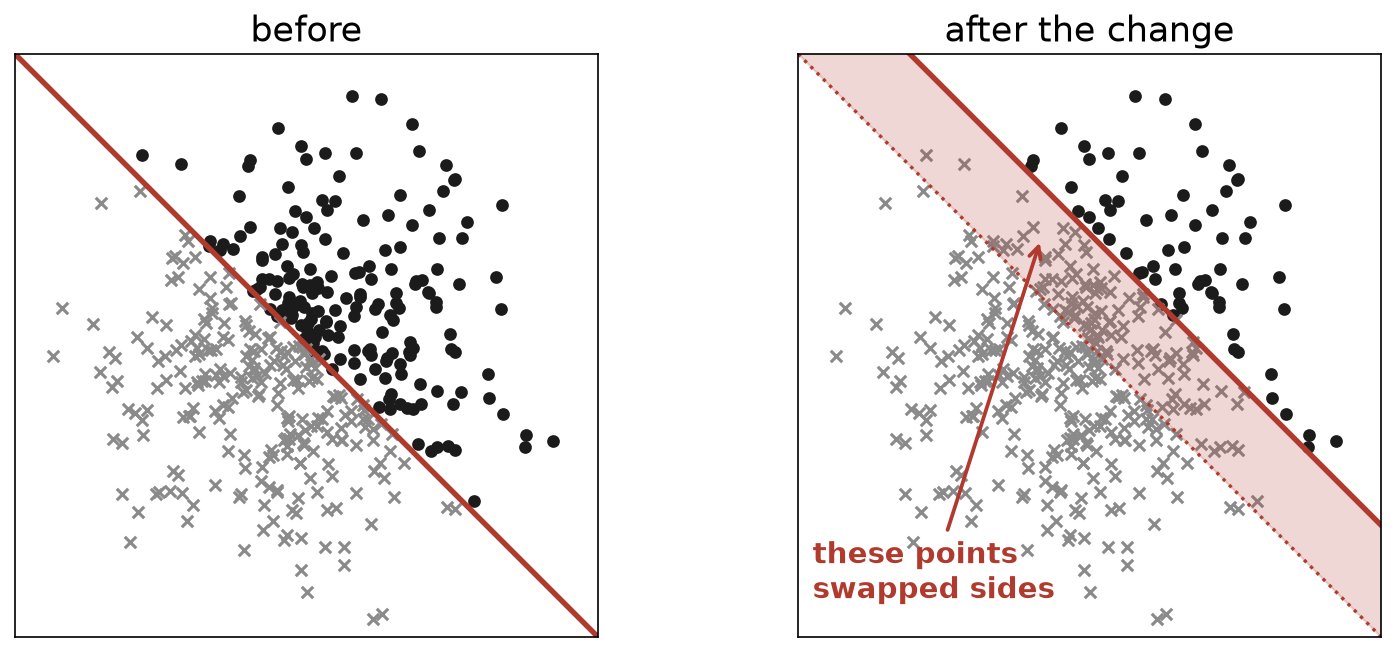
\includegraphics[height=0.60\textheight]{Fig_slide_drift.png}
  \end{center}
  \begin{center}
    A model trained on the left keeps predicting, confidently, and is now
    \alert{wrong on the shaded band}.
  \end{center}
  \note{First, the phenomenon. A model learns a rule: this input goes with
    that answer. Then the world changes and the rule no longer holds. That
    is concept drift, and here is the cleanest version of it, the one we
    simulate. Two inputs, a straight boundary, a label on each side. The
    change moves the boundary, and nothing else. Only the shaded band has
    swapped sides, and a model trained before is now wrong on it.}
\end{frame}

% ---------------------------------------------------------------- 33 s
\begin{frame}{Defence one: a model that repairs itself}
  \begin{center}
    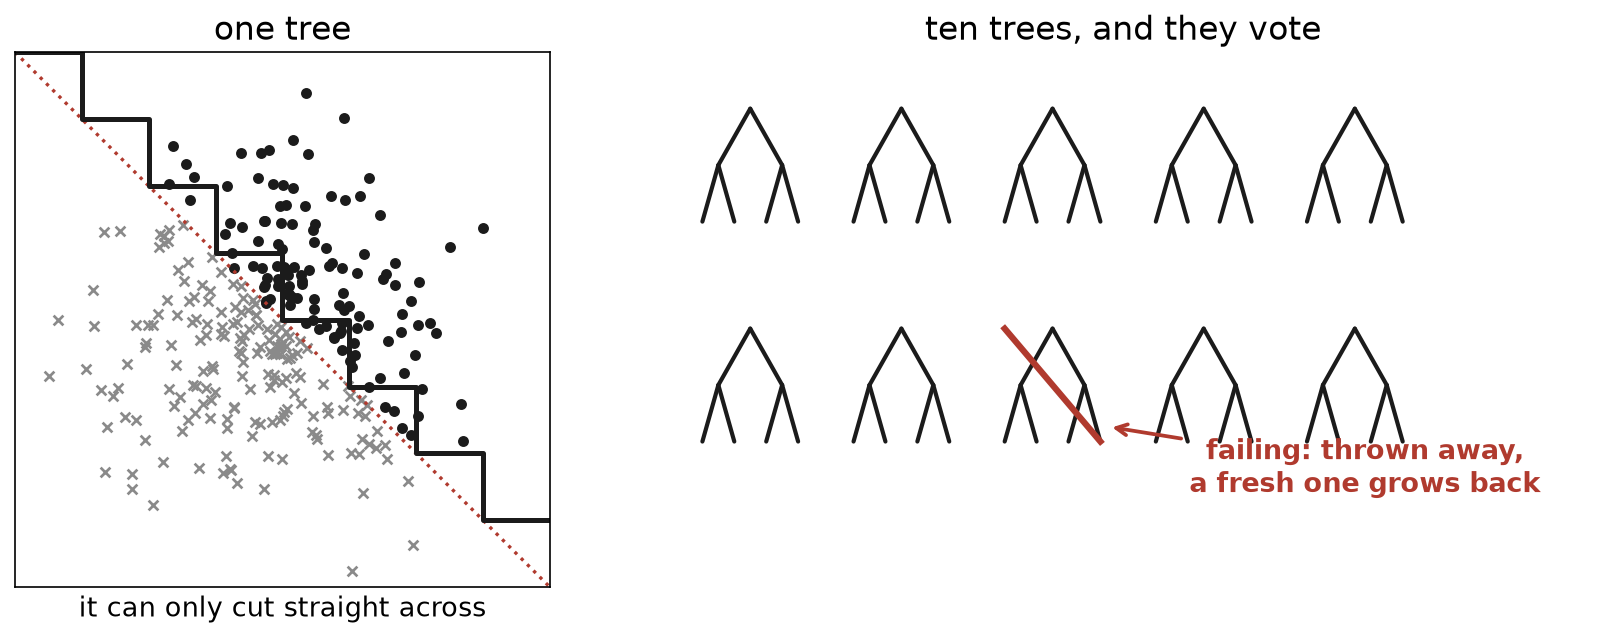
\includegraphics[width=0.94\textwidth]{Fig_slide_foret.png}
  \end{center}
  \vspace{-0.2em}
  \begin{center}
    This is the \alert{Adaptive Random Forest}. Ten trees, replaced one at a
    time.
  \end{center}
  \note{The first defence repairs itself. Its building block is a decision
    tree: it cuts the picture straight across, so a slanted boundary can
    only be approximated by a staircase. One tree is fragile, so ten of them
    vote. That is the Adaptive Random Forest, the model we study. A tree
    whose answers go wrong is thrown away, and a fresh one grows in its
    place. Ten trees, replaced one at a time.}
\end{frame}

% ---------------------------------------------------------------- 25 s
\begin{frame}{Defence two: a watchdog that raises the alarm}
  \begin{center}
    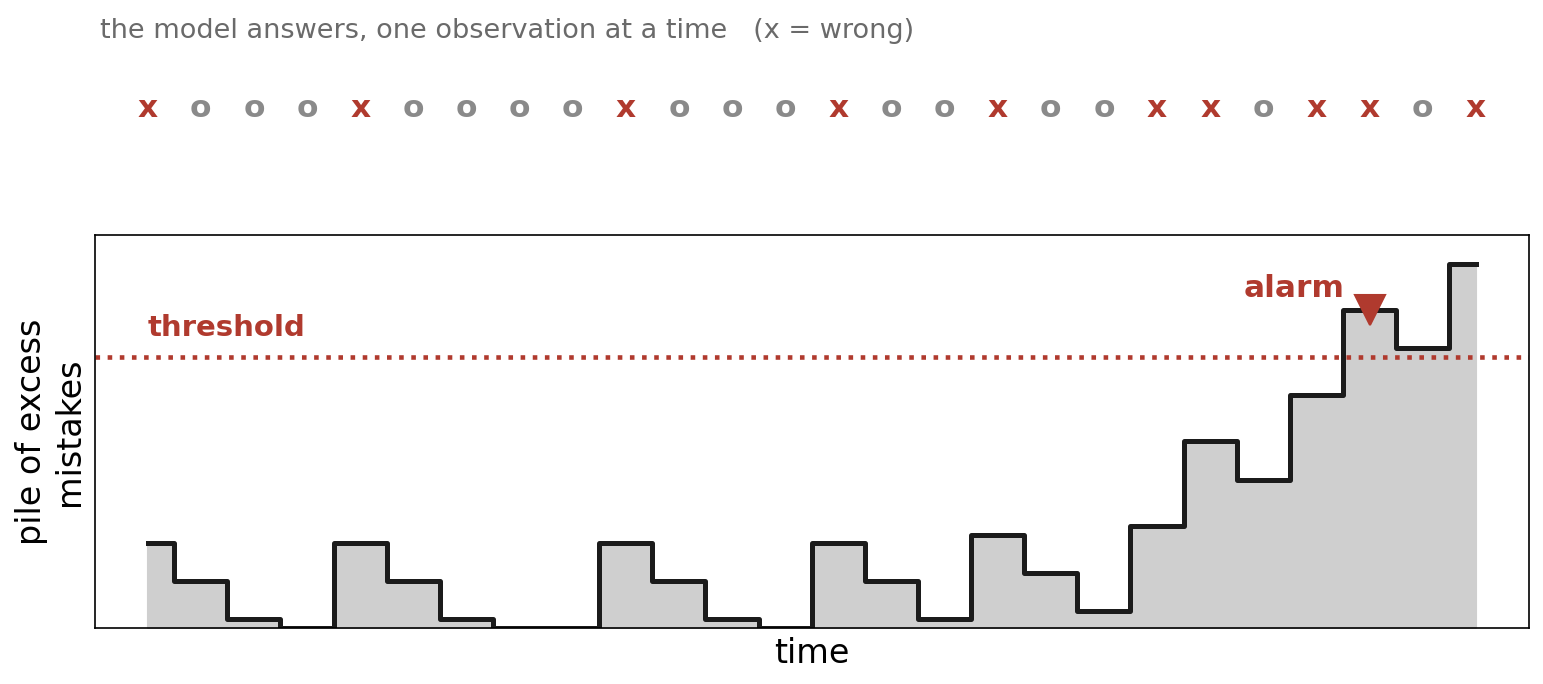
\includegraphics[width=0.94\textwidth]{Fig_slide_watchdog.png}
  \end{center}
  \vspace{-0.2em}
  \begin{center}
    Two communities, two tools, \alert{never measured against each other}.
  \end{center}
  \note{The second defence comes from a different community. A watchdog
    keeps a pile of the model's excess mistakes. While the model does well
    the pile falls back to zero; let the mistakes come and it grows, until
    it crosses a threshold and calls a human. That alarm is the only thing a
    human ever sees. Two communities, two tools, never measured against each
    other.}
\end{frame}

% ---------------------------------------------------------------- 35 s
\begin{frame}{Put them together, and they cancel out}
  \begin{center}
    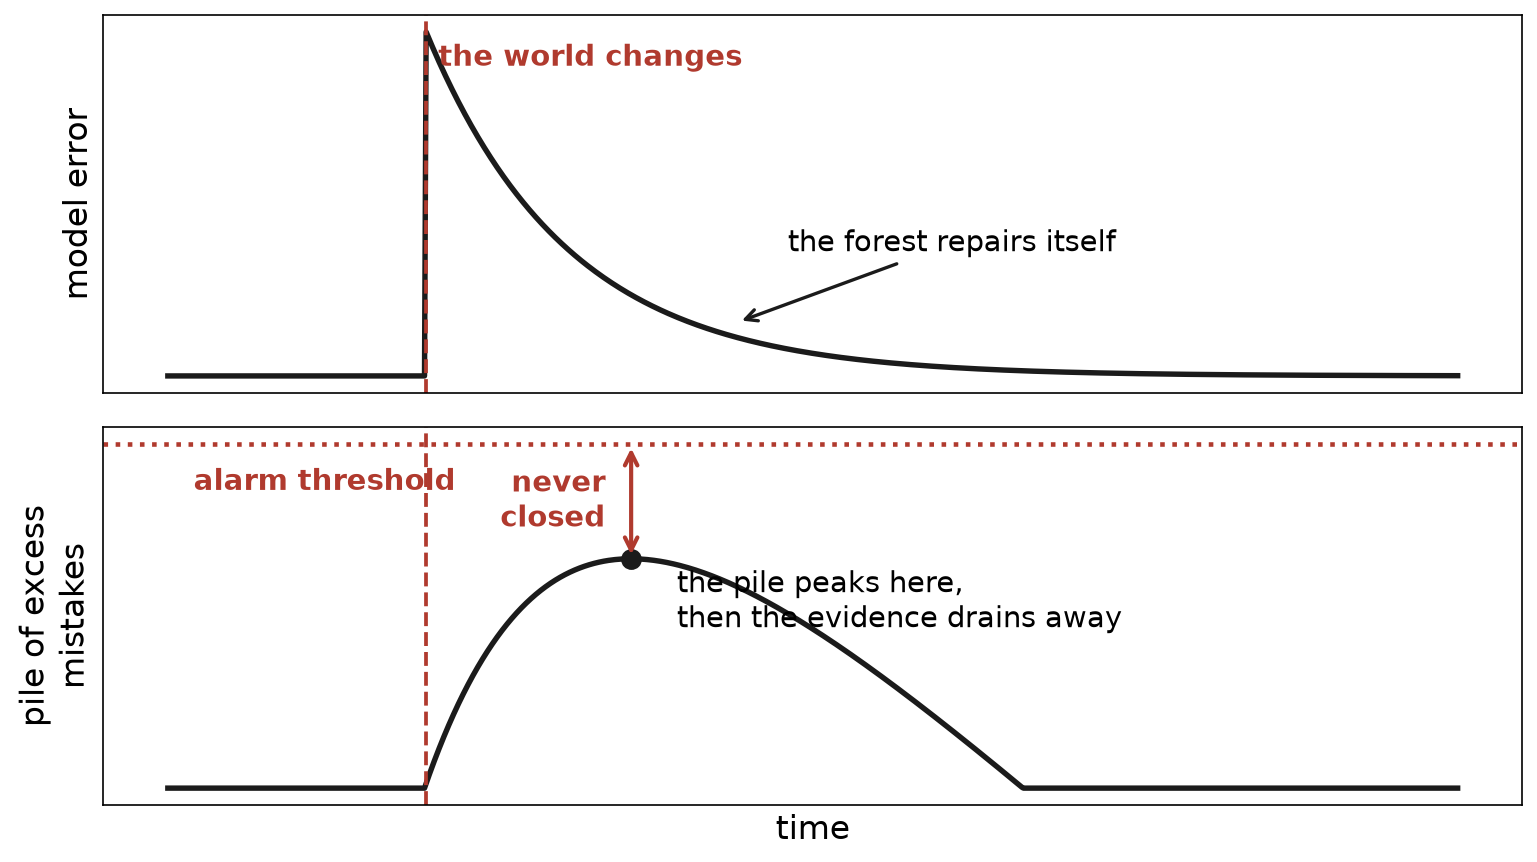
\includegraphics[height=0.70\textheight]{Fig_slide_mecanisme.png}
  \end{center}
  \vspace{-0.4em}
  \begin{center}
    \small schematic
  \end{center}
  \note{Put the two together, and they cancel out. The boundary moves, the
    mistakes begin, and the pile starts climbing. But the forest repairs
    itself, the mistakes stop, and the pile drains back to zero without ever
    reaching the threshold. The repair erased the evidence. The better the
    model fixes itself, the more surely the alarm stays silent.}
\end{frame}

% ---------------------------------------------------------------- 34 s
\begin{frame}{Why not just lower the threshold?}
  \begin{center}
    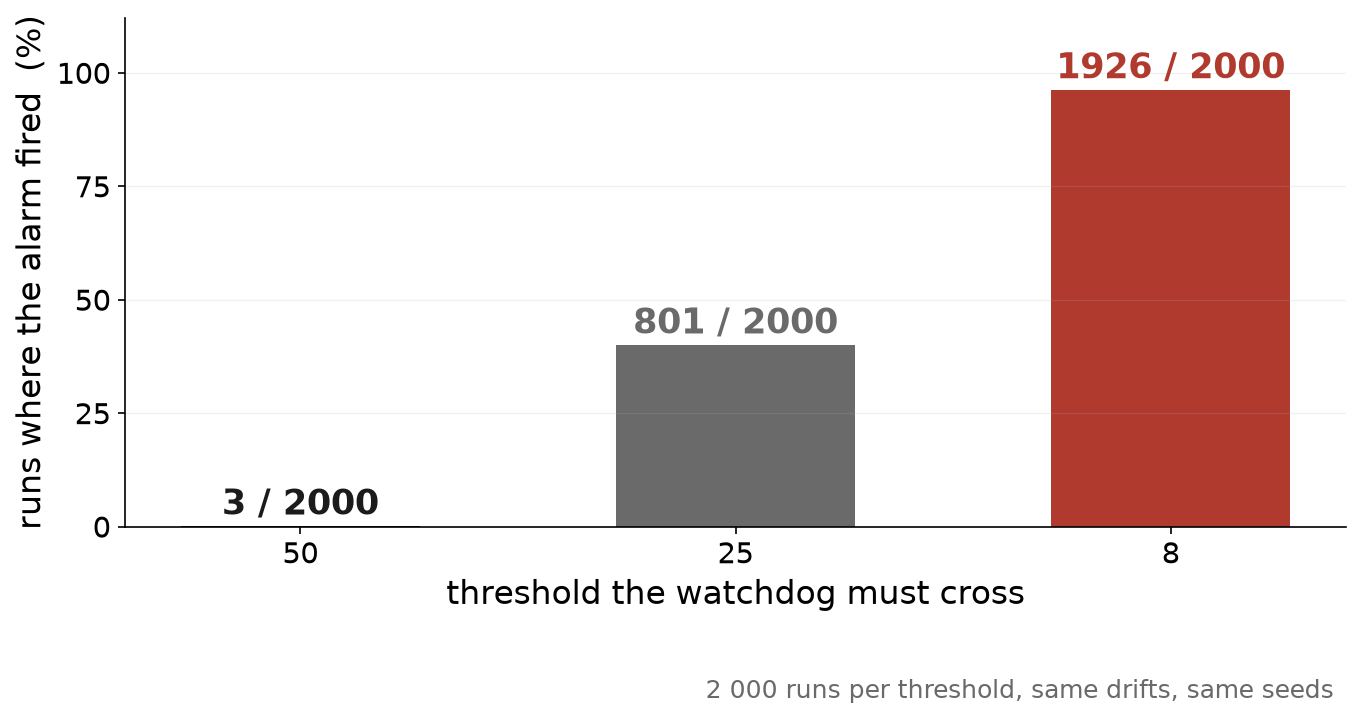
\includegraphics[width=0.80\textwidth]{Fig_slide_seuils.png}
  \end{center}
  \vspace{-0.3em}
  \begin{center}
    A low threshold also fires when \alert{nothing has happened}, and an
    alarm that cries wolf gets switched off.
  \end{center}
  \note{Does the alarm ever fire? That depends on the threshold. We re-ran
    the benchmark at three settings, two thousand runs each. At the highest
    it fired three times out of two thousand. Lower it, and it fires almost
    every time. So why not lower it? Because a low threshold also fires when
    nothing happened, and an alarm that cries wolf gets switched off. The
    setting quiet enough to be trusted is the one that never sees the
    drift.}
\end{frame}

% ---------------------------------------------------------------- 33 s
\begin{frame}{Our contribution: when is the forest actually repaired?}
  \begin{center}
    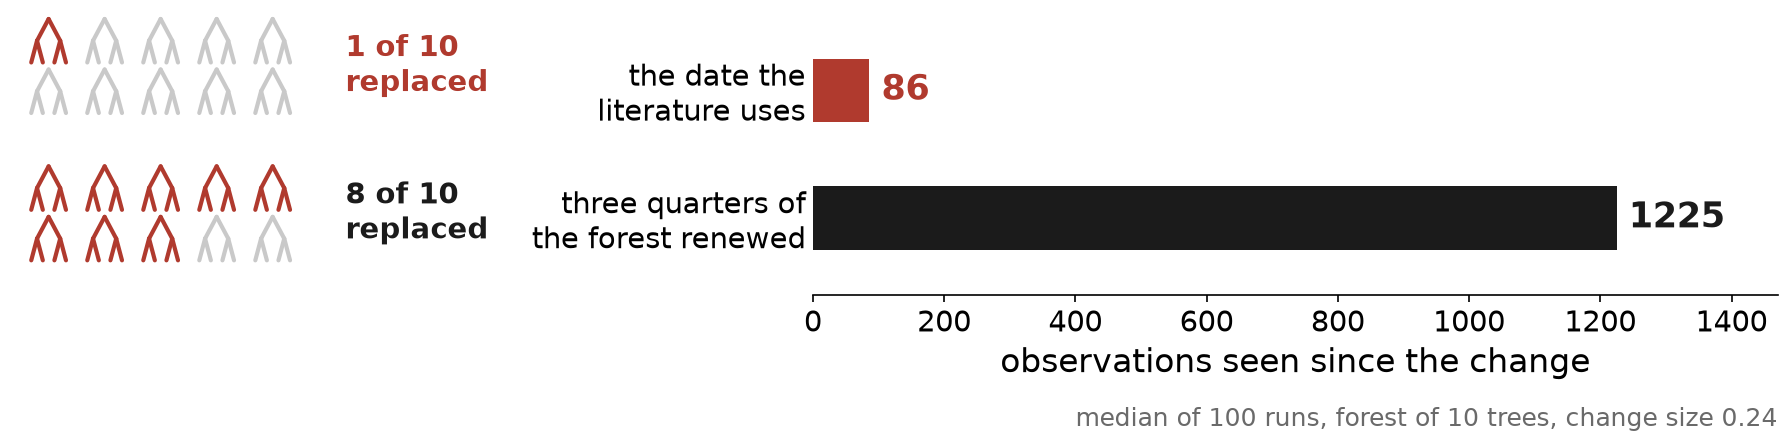
\includegraphics[width=\textwidth]{Fig_slide_deux_horloges.png}
  \end{center}
  \vspace{0.1em}
  \begin{center}
    \alert{\large The accepted date fires at the \emph{first} tree. It times
    the start of a repair, not its end.}
  \end{center}
  \note{It is a race, so we have to time both runners. Timing the alarm is
    easy. Timing the repair is where we found something. The literature has
    a standard date for it, and that date turns out to be the moment the
    very first tree out of ten is replaced. Wait until three quarters of the
    forest has actually been renewed, and you wait roughly ten times longer.
    That stopwatch times the start of a repair, not its end, and it is wrong
    always in the same direction.}
\end{frame}

% ---------------------------------------------------------------- 22 s
\begin{frame}{Where we stand}
  \begin{itemize}
    \item The paradox is \alert{real and reproducible}, and we can say when
          the evidence falls short of what the alarm needs.
    \item The clock the field relies on is \alert{biased, always the same
          way}. Every conclusion drawn from it inherits that bias.
    \item \textbf{Next}: watch the model and the watchdog on one common
          clock, and turn this into advice a practitioner can use.
  \end{itemize}
  \vfill
  \begin{center}
    \large Thank you.
  \end{center}
  \note{Where we stand. The paradox is real and reproducible. The clock the
    field relies on is biased, always the same way, so every conclusion
    drawn from it inherits that bias. What remains is to turn this into
    advice a practitioner can use. Thank you.}
\end{frame}

\end{document}
